\documentclass{article}
% \usepackage[spanish]{babel}
% \usepackage[utf8]{inputenc}
% \usepackage[backend=biber]{biblatex}
% \bibliography{referencias}
% Language setting
% Replace `english' with e.g. `spanish' to change the document language
\usepackage[spanish]{babel}

% Set page size and margins
% Replace `letterpaper' with `a4paper' for UK/EU standard size
\usepackage[letterpaper,top=2cm,bottom=2cm,left=3cm,right=3cm,marginparwidth=1.75cm]{geometry}

% Useful packages
\usepackage{amsmath}
\usepackage{graphicx}
\usepackage[colorlinks=true, allcolors=blue]{hyperref}
\usepackage{fancyhdr}
\usepackage[usenames]{color}
\usepackage{amssymb}

\title{Manual de instalación. ANEXO 1}
\author{YOLANDA MORALES ZAMORA}

\begin{document}
\maketitle

\begin{abstract}
En este documento se presenta los pasos a seguir para la instalación de la aplicación objeto de este proyecto.
Nombre del proyecto: Knowbuysell.
Framework utilizado: Laravel, el framework de los artesanos de la web.
Lenguaje de programación: PHP

\end{abstract}
\definecolor{Micolor1}{RGB}{193,124,250}
% \textcolor{Micolor1}{Comienzo Texto prueba pendiente de modificar }

\section{Introduction}
% \href{https://www.overleaf.com/learn}{help library}, or head to our plans page to \href{https://www.overleaf.com/user/subscription/plans}{choose your plan}.
\subsection{Introducción del proyecto}
% Breve introducción justificando los motivos para la elaboración del proyecto y/o necesidades en el sector productivo para la elaboración del mismo. Se pueden añadir también las ventajas que puede tener el uso del proyecto
En el documento principal, en el informe KNOWBUYSELL, ya se indica que el objetivo principal es obtener información por parte del usuario y del administrador, y cada uno de ellos obtiene benenficios, el usuario para poder organizar sus gastos y el administrador para ofrecer productos de interés al usuario y así aumentar las ventas y la atención al usuario para ofrecer lo que más le interese.
\subsection{Propósito}
% Especificar características del proyecto y uso una vez desarrollado.
Una vez desarrollado el proyecto, el administrador va a poder ofrecer los productos de la categoría que más interesa al usuario.
\subsection{Objetivos del proyecto}
En cuanto a los objetivos del proyectos nos referimos al informe KNOWBUYSELL, al que complemente este informe.
\subsection{Coste del proyecto}
En cuanto a los coster del proyectos nos referimos al informe KNOWBUYSELL, al que complemente este informe.
% \textcolor{Micolor1}{Fin Texto prueba pendiente de modificar }
\section{Manual de Instalación}
% (Detallad paso a paso la instalación de las aplicaciones necesarias para desarrollar dicha aplicación con los apartados que veáis necesarios)
\subsection{Información básica Laravel \& PHP}
Laravel es un framework de desarrollo web de código abierto escrito en PHP. Fue creado por Taylor Otwell y se lanzó por primera vez en 2011. 
Basado en el patrón de desarrollo MVC (modelo-vista-controlador), que implica la modularización de los componentes y partes del software. Esto te permite separar elementos de la vista y del diseño, de las estructuras de datos, y del código orientado a la lógica. Separa las aplicaciones en pares modulares, más pequeñas, que pueden modificarse sin alterar los componentes.
PHP es el lenguaje del lado del servidor, es decir, no corre directamente como lo hace HTML, CSS o Javascript, sino que necesita un servidor web para ser ejecutado, como puede ser Apache, entre sus características es un lenguaje con facilidad para crear un servidor y levantar el sitio.
Investigando hemos descubierto que existen distintos paquetes que permiten crear un servidor de desarrollo con varias herramientas que serán útiles, como por ejemplo: EasyPHP, paquete completo que contiene en su instalación diversas herramientas para el desarrollador, entre ellas, el lenguaje PHP, MySQL, el motor de bases de datos no relacional MongoDB, los servidores Apache y Ngimx, Xdebug, el gestor de bases de datos PostgreSQL y WordPress, entre otras tecnologías interesantes.
Xampp permite instalar rápidamente PHP, MySQL, Apache y TomCat (servidor para lenguaje Java en la web).
ORM (Object Relational Mapping) o mapeo de objetos realacional, es la técnica por medio de la cual se pueden abstraer las consultas SQL o métodos de clases.
Los modelos en el MVC son clases que permiten moldear cómo serán los objetos de las clases de bases de datos y cómo puede ejecutarse operaciones sobre ellos. 
El ORM de Laravel es ELOQUENT, componente que permite abstraerse de las consultas SQL tradicionales y trabajar con bases de datos de manera mucho más simple.
También existe lo que se conoce como Scaffolding, técnica provista por varios entornos de trabajo modernos, que se basan en generar componentes de software de manera automática para facilitar tareas al desarrollador, creando controladores, vistas, modelos y migraciones, entre muchas otras cosas.
\subsection{Recorrido simplificado de instalaciones}
\subsubsection{Laravel}
¿Qué es Laravel? Laravel es un framework de desarrollo de aplicaciones web PHP de código abierto, que se utiliza para crear aplicaciones web robustas, escalables y seguras. 
Desarrollado por Taylor Otwell en 2011 y desde entonces ha crecido en popularidad debido a su facilidad de uso, modularidad y amplia gama de características avanzadas.
Laravel utiliza el patrón de diseño MVC (Modelo Vista Controlador) para separar la lógica de presentación de la lógica de negocio y de acceso a los datos, lo que hace que sea fácil de mantener y escalar. Además, Laravel cuenta con un conjunto completo de características como rutas, controladores, vistas, migraciones de bases de datos, autenticación, envío de correos electrónicos, colas, programación de tareas y más, lo que permite a los desarrolladores construir aplicaciones web de alta calidad de manera rápida y eficiente.
Entre las principales características de Laravel se encuentran la simplicidad y la elegancia del código, la documentación extensa y clara, la robustez de seguridad, la facilidad de integración con bibliotecas y paquetes de terceros y la capacidad de crear API y aplicaciones de tiempo real. Laravel es una excelente opción para desarrollar proyectos web empresariales y de cualquier otro tipo.
¿Qué necesitamos para instalar Laravel?
Para empezar:
\begin{itemize}
    \item XAMPP
    \item COMPOSER
    \item CMD ó GIT BASH
    \item COMANDOS (Instalación y comprobación).
    \item VSC
\end{itemize}
En la cita número \cite{instalacionLaravel} de la referencia al final del documento puede localizar el enlace de tutorial para la instalación de Laravel.
\begin{enumerate}
    \item     XAMPP 
No vamos a profundizar en este apartado, porque ya lo hemos realizado en trabajos anteriores, pero sí podemos indicar que la ubicación desde dónde podemos descargarlo, es la dirección que indicamos a continuación. Enlace \url{https://www.apachefriends.org/es/download.html}

    \item     COMPOSER: 
        \begin{enumerate}
            \item ¿qué es Composer?
Composer es una herramienta de gestión de dependencias para PHP que permite instalar, actualizar y administrar las bibliotecas y paquetes de terceros que una aplicación PHP necesita para funcionar.

Con Composer, los desarrolladores pueden especificar las dependencias de sus proyectos PHP en un archivo llamado "composer.json" y Composer se encarga de descargar e instalar las bibliotecas y paquetes necesarios en la estructura de directorios del proyecto. Además, Composer garantiza que todas las dependencias estén en las versiones correctas y maneja los conflictos entre dependencias.

De esta manera, Composer facilita la gestión y el mantenimiento de los proyectos PHP, ya que los desarrolladores no tienen que preocuparse por descargar y actualizar manualmente las bibliotecas y paquetes de terceros que sus proyectos requieren. En lugar de eso, pueden centrarse en escribir el código de su aplicación y dejar que Composer maneje las dependencias.
En resumen, Composer es una herramienta esencial para cualquier proyecto PHP moderno, ya que permite una gestión de dependencias fácil y automatizada, lo que ahorra tiempo y reduce la posibilidad de errores.
            \item Instalación de Composer de forma Manual a través de su interfaz.
Descargamos el fichero desde la ruta: \url{https://getcomposer.org/download/}
Una vez descargado seguimos las siguientes pautas para su instalación, siempre teniendo encuenta las referencias de descarga \cite{descargaComposer} e instalación \cite{instalaComposer} de Composer en las siguientes Figuras \ref{fig:01}, \ref{fig:02}, \ref{fig:03}, \ref{fig:04}, \ref{fig:05} y \ref{fig:06} podemos ver el proceso.


\begin{figure}[!]
\centering
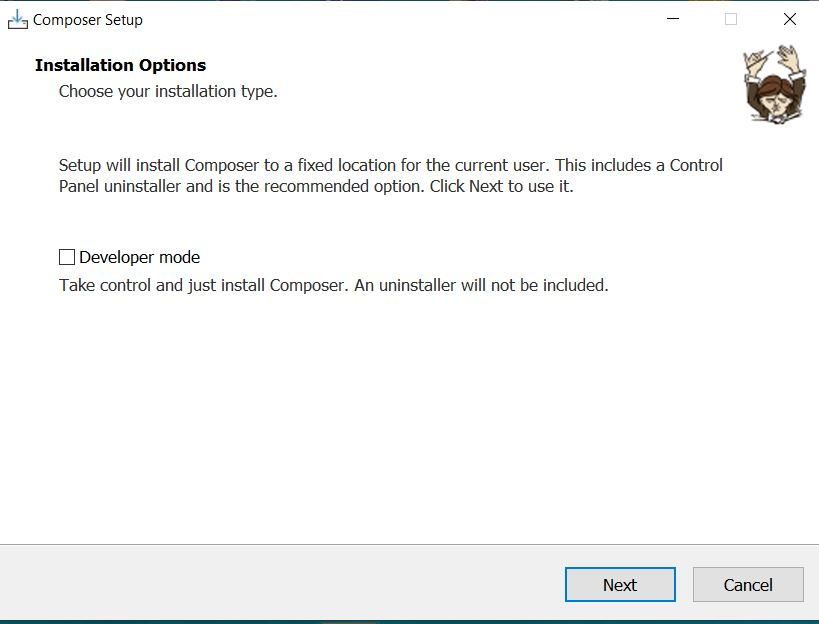
\includegraphics[width=12cm]{ImagenComposer1.jpg}
\caption{\label{fig:01} Instalación Composer. Paso 1}
\end{figure}

\begin{figure}[!]
\centering
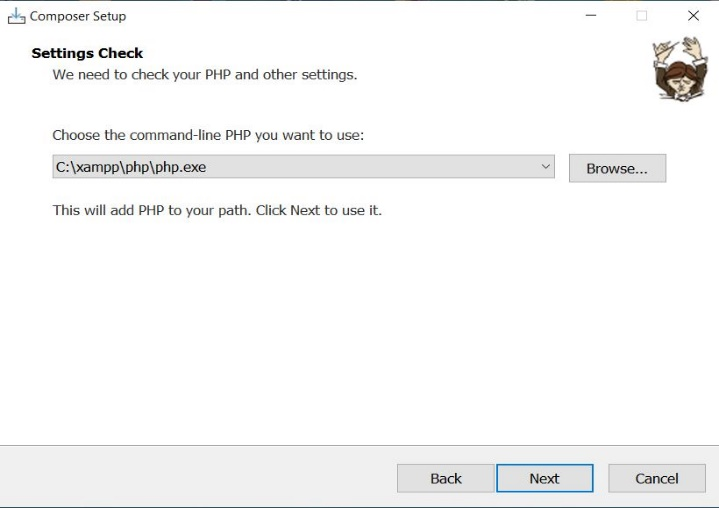
\includegraphics[width=12cm]{ImagenComposer2.jpg}
\caption{\label{fig:02} Instalación Composer. Paso 2}
\end{figure}

\begin{figure}[!]
\centering
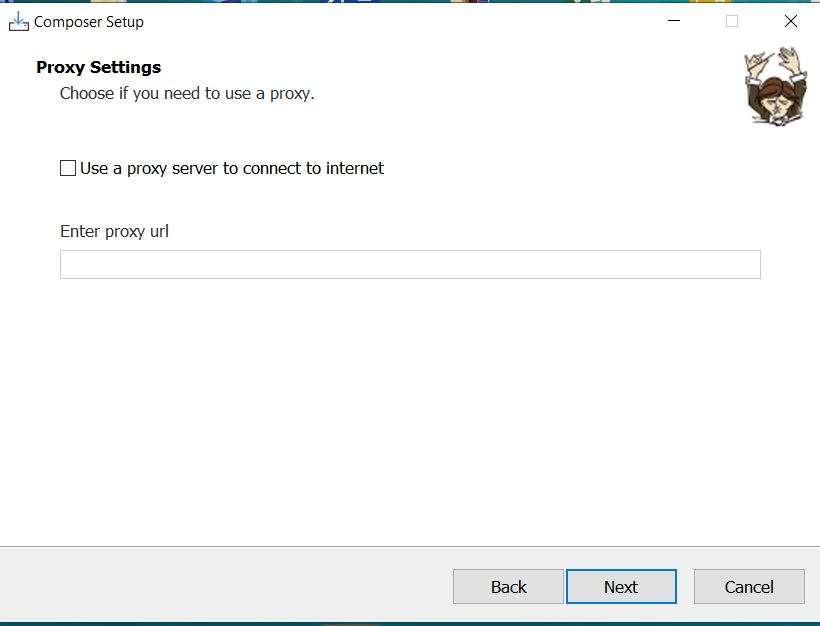
\includegraphics[width=12cm]{ImagenComposer3.jpg}
\caption{\label{fig:03} Instalación Composer. Paso 3}
\end{figure}

\begin{figure}[!]
\centering
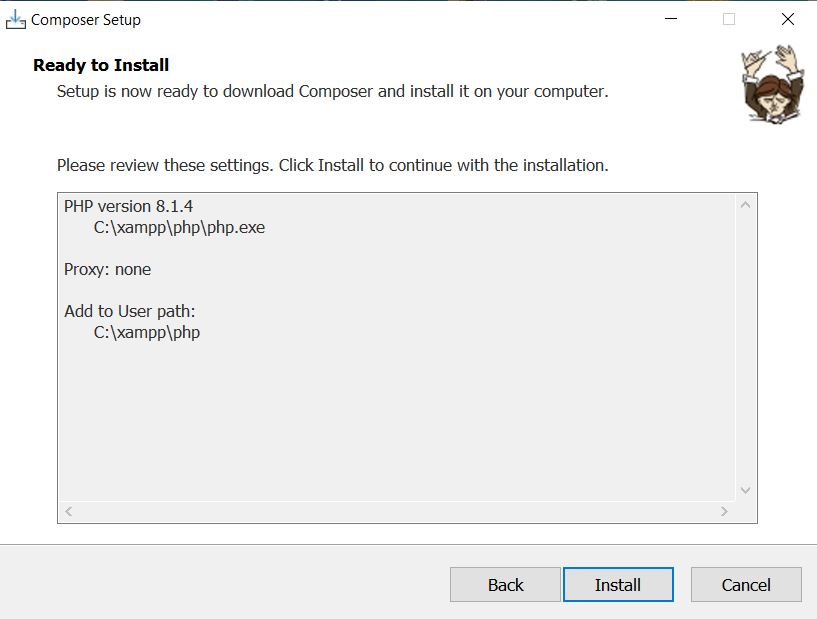
\includegraphics[width=12cm]{ImagenComposer4.jpg}
\caption{\label{fig:04} Instalación Composer. Paso 4}
\end{figure}

\begin{figure}[!]
\centering
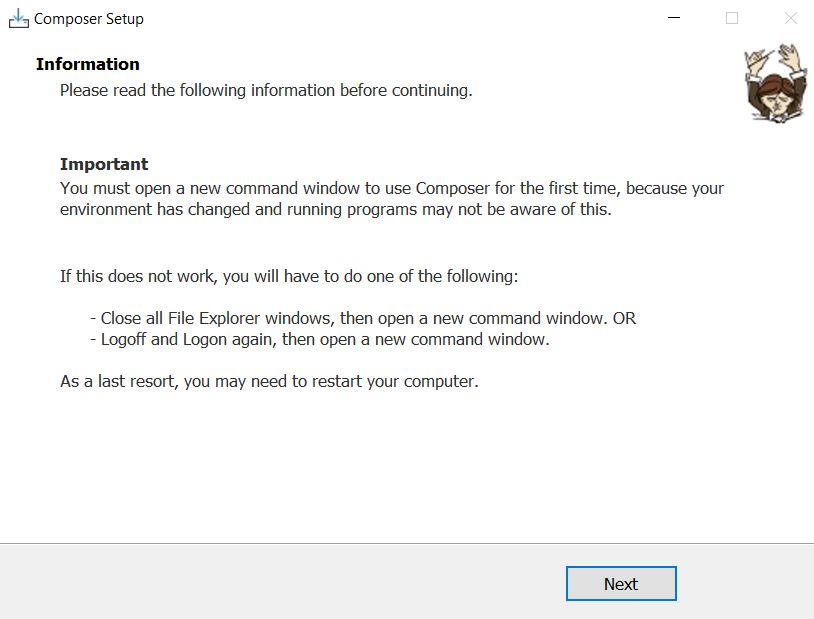
\includegraphics[width=12cm]{ImagenComposer5.jpg}
\caption{\label{fig:05} Instalación Composer. Paso 5}
\end{figure}

\begin{figure}[!]
\centering
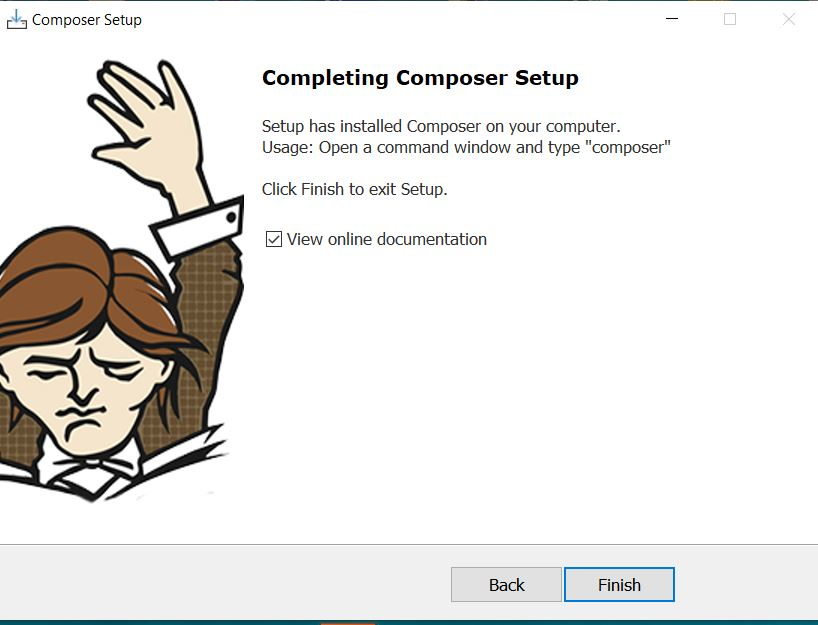
\includegraphics[width=12cm]{ImagenComposer6.jpg}
\caption{\label{fig:06} Instalación Composer. Paso 6}
\end{figure}


En las Figuras \ref{fig:07} y \ref{fig:08} comprobamos que la instalación se ha realizado de forma correcta: ¿Cómo lo hacemos? Abrimos el terminal de windos con ‘cmd’ y una vez en él escribimos ‘Composer’ ejecutamos y este es el resultado que obtenemos para comprobar que se ha instalado de forma correcta.

\begin{figure}[!]
\centering
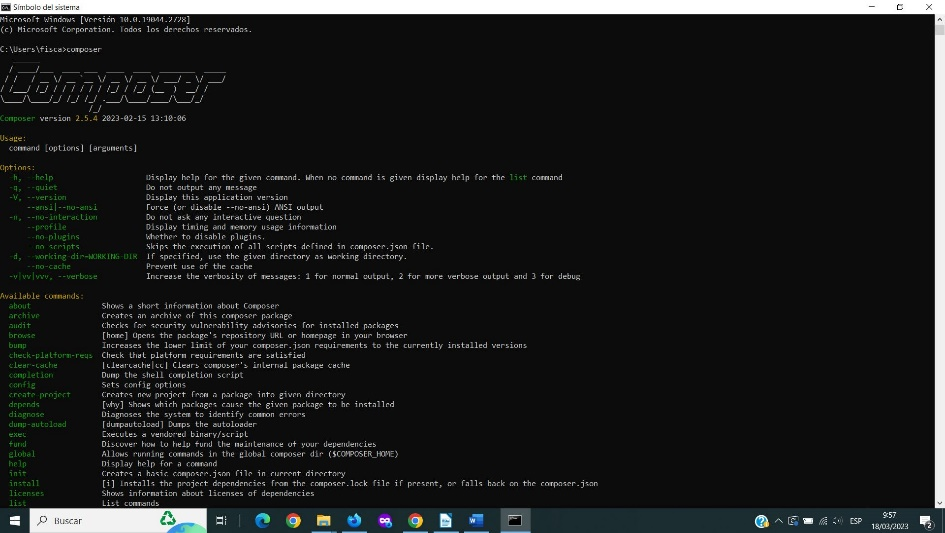
\includegraphics[width=12cm]{ImagenComposer7.jpg}
\caption{\label{fig:07} Comprobación Composer. Paso 7}
\end{figure}

\begin{figure}[!]
\centering
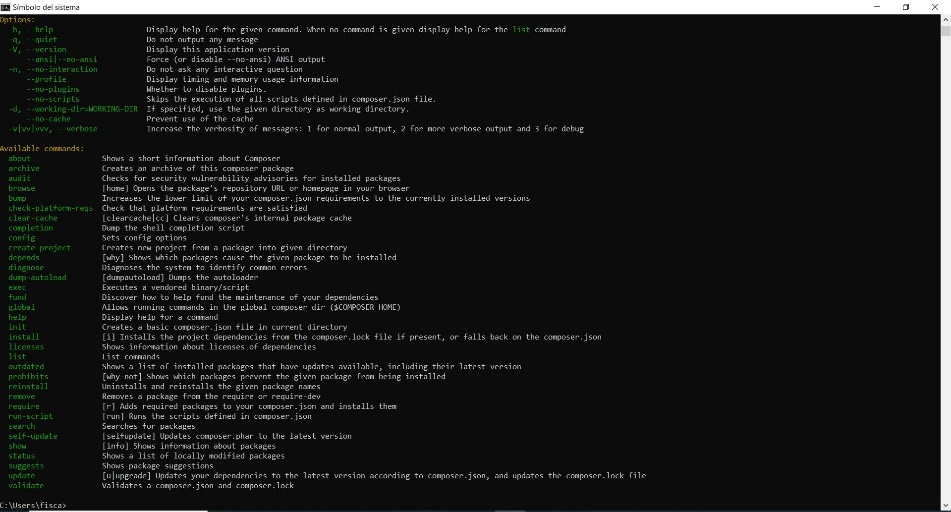
\includegraphics[width=12cm]{ImagenComposer8.jpg}
\caption{\label{fig:08} Comprobación Composer. Paso 8}
\end{figure}


            \item  Comandos para instalar Composer a través de comandos.
Tutorial explicativo para hacerlo en S.O. Windows \url{https://www.youtube.com/watch?v=yp04wvbAJPs}

Comandos a utilizar para la instalación de Comproser los podemos comprobar en las Figuras \ref{fig:08} y \ref{fig:09}.

\begin{figure}[!]
\centering
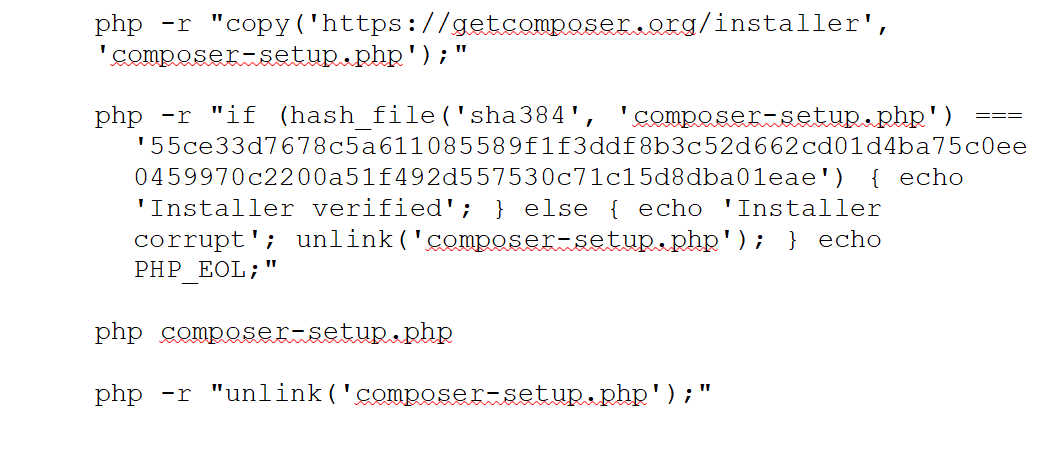
\includegraphics[width=12cm]{Comandos9.png}
\caption{\label{fig:09} Comandos para instalación  }
\end{figure}

\begin{figure}[!]
\centering
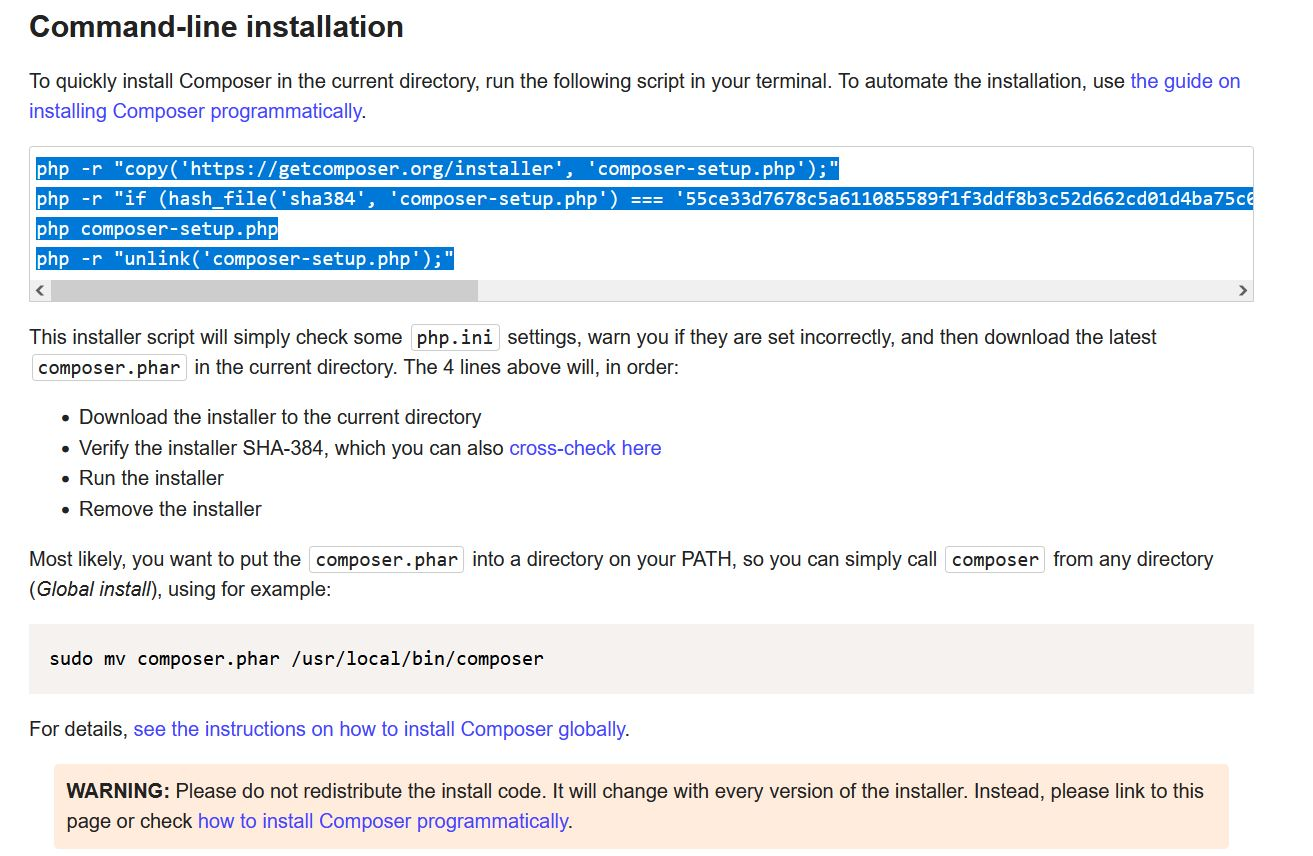
\includegraphics[width=12cm]{Comandos10.jpg}
\caption{\label{fig:10} Comandos para instalación e indicaciones }
\end{figure}

        \end{enumerate}


\item Documentación Laravel: comandos instalación Laravel.
Los comandos tanto para la instalación de Laravel, como para consultar su documentación lo podemos encontrar en el siguiente enlace: \url{http://laravel.com/docs/11.x}, más referencias relacionadas en \cite{docLaravel} y
\cite{docLaravelviews}.

Comandos de instalación: 


\textbf{Composer create-project laravel/laravel  ProjecNam} 

‘OR’ 

\textbf{Composer global require laravel/installer}\\
\\

\item  Nombre del proyecto: comandos para crear proyecto
\begin{enumerate}
    \item  Comandos para crear proyecto:
    
            \textbf{laravel new ProjecName}
    \item  Comprobación del proyecto creado. 

        \textbf{http://localhost/s1project/public/}
\end{enumerate}

Al igual que Python o Javascript tiene paquetes como pip o npm, en Composer encontramos un gestor de paquetes y dependencias por excelencia de PHP.
Cuando Xampp y Composer ya se han instalado, nos situamos en el terminal de de VSC (ctrl+ñ) y utilizamos los siguientes comandos: 

\textbf{php-v}

\textbf{composer –version}

Nos servirán para saber qué versión de php tenemos instalada al igual qué versión de Composer.



\item  Visual Studio Code.
Hemos realizado la instalación de paquetes necesarios para Laravel, a través de la terminal de VSC.
Son beneficiosas determinadas extensiones para instalar en VSC, como las siguientes:
\begin{itemize}
    \item Laravel snippets
    \item Laravel Blade format
    \item Laravel Blade Snippets
    \item Laravel go to view
    \item Php intelliphense
    \item Spanish Language Pack for VSC
    \item Tailwind CSS intellisense
    \item Alpine.js intellisense
    \item Github Copilot
\end{itemize}

\subsubsection{¿Cuáles son las características principales?}
Laravel es un framework de PHP moderno y robusto que tiene varias características principales que lo hacen popular y ampliamente utilizado en la comunidad de desarrollo web. A continuación, se presentan algunas de las características principales de Laravel:

Enrutamiento elegante y fácil de usar: Laravel proporciona una sintaxis de enrutamiento fácil de usar que permite definir rutas con parámetros, prefijos y restricciones.

Capacidad de autenticación integrada: Laravel viene con características integradas de autenticación, lo que facilita la implementación de la autenticación y autorización en aplicaciones web.

ORM (Mapeo objeto-relacional) integrado: Laravel incluye Eloquent, un ORM integrado que permite la interacción con bases de datos de forma sencilla y natural, utilizando una sintaxis elegante y expresiva.

Sistema de plantillas Blade: Laravel proporciona un sistema de plantillas llamado Blade que permite crear vistas de forma sencilla y expresiva. Blade incluye características como herencia de plantillas, control de flujo y directivas personalizadas.

Consola de Artisan: Laravel viene con una herramienta de línea de comandos llamada Artisan que permite la creación de migraciones, modelos, controladores, pruebas y más. Artisan también permite la personalización de comandos para automatizar tareas repetitivas.

Facilita la creación de API: Laravel facilita la creación de API mediante el uso de controladores de recursos y el soporte para autenticación API mediante tokens.

Soporte para caché: Laravel proporciona una API de caché simple y expresiva que permite almacenar en caché datos de forma sencilla.

Arquitectura MVC: Laravel sigue una arquitectura MVC (Modelo-Vista-Controlador) que permite separar la lógica de la aplicación en diferentes capas.

Estas son solo algunas de las características principales de Laravel que lo hacen popular y ampliamente utilizado en la comunidad de desarrollo web. Laravel también cuenta con una amplia documentación y una comunidad activa de desarrolladores, lo que lo hace aún más atractivo para el desarrollo de aplicaciones web.

\subsubsection{Se basa en la estructura MVC}
MVC significa "Modelo-Vista-Controlador" y es un patrón de diseño de software comúnmente utilizado en el desarrollo de aplicaciones web. Es utilizado por Laravel para organizar la lógica de la aplicación en diferentes capas, lo que permite separar las responsabilidades y facilita la gestión del código.

En Laravel, el modelo representa los datos y la lógica de la aplicación relacionados con esos datos. El controlador se encarga de procesar las solicitudes del usuario y controlar la lógica de negocio de la aplicación. La vista es responsable de mostrar los datos al usuario y proporcionar una interfaz de usuario interactiva.

El modelo, la vista y el controlador se comunican entre sí mediante una serie de reglas y convenciones que Laravel establece. Por ejemplo, el controlador puede llamar al modelo para recuperar los datos de la base de datos y luego pasar esos datos a la vista para que se muestren al usuario.

La arquitectura MVC de Laravel permite una mayor modularidad y flexibilidad en el desarrollo de aplicaciones web. También facilita la colaboración en equipo, ya que cada desarrollador puede trabajar en una capa diferente de la aplicación sin afectar el trabajo de los demás. Ver esquema en Figura \ref{fig:011}

Enlaces importantes de tutoriales para Laravel: cómo hacer un Hola Mundo en Laravel ver referencia \cite{HolaMundoLaravel}, cómo hacer un registro y un login el Laravel\cite{registroYlogin}, cómo hacer un CRUD en Laravel \cite{CRUDLaravel}, cómo crear un proyecto en Laravel \cite{Laravel10CrearProyecto} y cómo entender las vistas en Laravel\cite{Laravel10Vistas}


\begin{figure}[!]
\centering
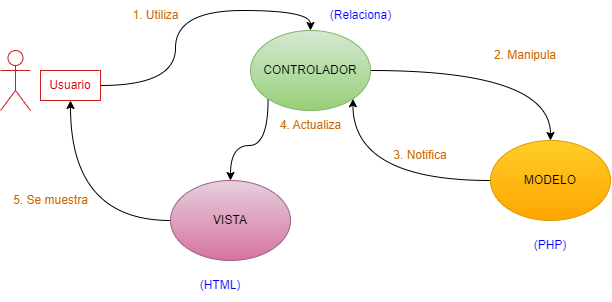
\includegraphics[width=12cm]{mvcEsquema.png}
\caption{\label{fig:011} Esquema Modelo Vista Controlador }
\end{figure}

\subsubsection{¿Qué es un ORM? ¿Cuál es el ORM que utiliza Laravel por defecto?}
Un ORM (Object-Relational Mapping) es una técnica de programación que permite a los desarrolladores interactuar con una base de datos relacional utilizando objetos en lugar de sentencias SQL. En lugar de tener que escribir código SQL para cada operación de base de datos, los desarrolladores pueden trabajar con objetos en su lenguaje de programación, lo que simplifica el proceso de desarrollo y hace que el código sea más legible y mantenible.

En Laravel, el ORM por defecto es Eloquent. Eloquent es un ORM de alto rendimiento y fácil de usar que utiliza convenciones de nomenclatura para mapear modelos de objetos a tablas de base de datos y relaciones entre ellos. Con Eloquent, los desarrolladores pueden interactuar con sus bases de datos utilizando una sintaxis limpia y concisa en lugar de tener que escribir consultas SQL directamente. Eloquent admite una amplia gama de relaciones, como uno a uno, uno a muchos, muchos a muchos y polimórficas, y también incluye características avanzadas como la carga impaciente, el acceso a atributos, el control de versiones y la migración de esquemas de base de datos.

Eloquent es un ORM potente y fácil de usar que simplifica el acceso a la base de datos en Laravel, esto ayuda a que los desarrolladores puedan centrarse en el desarrollo de la lógica de la aplicación en lugar de preocuparse por la gestión de la base de datos.

\subsubsection{Analizar las partes consideradas más importantes del desarrollo.}
Hemos realizado una aplicación para que un usuario pueda registrarse y logarse a través de una página web, en dicha aplicación hemos utilizado lenguaje php, html, css y javascript en cuanto a las secciones de Servidor y Cliente.

La aplicación la hemos realizado con VSC, a través de su terminal hemos insertado los comandos más importantes como son: 

Crear proyecto laravel:  \textbf{laravel new ProjectName}\\
Levantar servidor: \textbf{php artisan serve}\\
Migrar tablas a nuestra base de datos de PhpmyAdmin: \textbf{php artisan migrate}\\
Nota: Para las migraciones en Laravel hemos consultado en \cite{docLaravelmigrations}\\
Crear controladores: \textbf{php artisan make:controller NameController}\\
Crear petición: \textbf{php artisan make:request NameRequest}\\

Nos vamos a la carpeta ‘htdocs’ dentro de la ruta de Xampp, y allí abrimos la consola y en ella ejecutamos: 

\textbf{composer create-project laravel/laravel mi-primer-app}  

Este comando se encarga de visitar el repositorio oficial de laravel en GitHub, para buscar la última versión estable del proyecto, y clona en tu pc o portátil una versión limpia en una carpeta con el nombre que coloques después de la instrucción “laravel/laravel”.
Instala también todas las dependencias necesarias para el framework.
El navegador es: localhost/mi-primer-app/public con el servidor Apache encendido en el panel de control (Xampp). Aparecerá la pantalla de laravel de su vista “welcome.blade.php”.
En el terminal si no estamos en la carpeta del proyecto, usamos el comando cd mi-primer-app y después php artisan serve.
El localhost es 8000
Además del VSC existen otro entorno de desarrollo integrado para PHP llamado PHPStorm que es de pago, excepto para las universidades.


Las carpetas y ficheros del proyecto realizado con Laravel sobre las que más hemos trabajado y considero más importantes, son:

\begin{itemize}
    \item -	App/Http/Controllers: (donde vamos a determinar las funciones importantes)
        \begin{itemize}
            \item ChartController.php
            \item CompraController.php
            \item Controller.php
            \item CookieController.php
            \item HomeController.php
            \item LoginController.php
            \item LogoutController.php
            \item RegisterController.php
            \item VentaController.php
            \item WelcomeController.php
        \end{itemize}
    \item App/Http/Requests:(peticiones para el logo y el registro)
        \begin{itemize}
            \item LoginRequest.php
            \item RegisterRequest.php
        \end{itemize}
    \item App/Models:(nuestras clases a tener en cuenta)
        \begin{itemize}
            \item Compra.php
            \item User.php
            \item Venta.php
        \end{itemize}
    \item Config:(para la configuración cuando se instalan paquetes para determinadas funciones)
        \begin{itemize}
            \item app.php
            \item auth.php
            \item charts.php
            \item database.php
            \item session.php
            \item view.php
        \end{itemize}
    \item Database/migrations:(a través de las migraciones podemos dar forma a nuestra base de datos MaríaDB)
        \begin{itemize}
            \item 2014\_10\_12\_000000\_create\_users\_table.php
            \item 2014\_10\_12\_100000\_create\_password\_reset\_tokens\_table.php
            \item 2019\_08\_19\_000000\_create\_failed\_jobs\_table.php
            \item 2019\_12\_14\_000001\_create\_personal\_access\_tokens\_table.php
            \item 2023\_05\_13\_230948\_create\_categoria\_table.php
            \item 2023\_05\_13\_232745\_create\_ventas\_table.php
            \item 2023\_05\_14\_031345\_eliminar\_tabla\_nombre\_de\_la\_tabla.php
            \item 2023\_11\_12\_211851\_create\_compras.php
            \item 2023\_11\_19\_182744\_create\_permission\_tables.php
            \item 2023\_11\_27\_162602\_create\_roles.php
        \end{itemize}
    \item Database/seeders:(aquí configuramos los roles de Administrador y usuario) 
        \begin{itemize}
            \item RoleSeeder.php
        \end{itemize}
    \item Public/assets/css:(aquí configuramos la parte cliente)
        \begin{itemize}
            \item Bootstrap.min.css
            \item Bootstrap.min.css.map
        \end{itemize}
    \item Public/assets/js: (también para usar js en nuestra parte cliente)
        \begin{itemize}
            \item Bootstrap.bundle.min.js
            \item Bootstrap.bundle.min.js.map
        \end{itemize}
    \item Resources/views/auth:(nuestras vistas, cómo vamos a ver las páginas)
        \begin{itemize}
            \item Login.blade.php
            \item Register.blade.php
        \end{itemize}
    \item Resources/views/charts:
        \begin{itemize}
            \item graficas.blade.php
        \end{itemize}
    \item Resources/views/compra:
        \begin{itemize}
            \item create.blade.php
            \item edit.blade.php
            \item form.blade.php
            \item index.blade.php
            \item pdf.blade.php
        \end{itemize}
    \item Resources/views/home:
        \begin{itemize}
            \item Index.blade.php
        \end{itemize}
    \item Resources/views/layouts/partials:
        \begin{itemize}
            \item Messages.blade.php
            \item Navbar.blade.php
        \end{itemize}
    \item Resources/views/layouts:
        \begin{itemize}
            \item app-master.blade.php
            \item app-master.blade.php
            \item base.blade.php
        \end{itemize}
    \item Resources/views:
        \begin{itemize}
            \item compras.blade.php
            \item departamentos.blade.php
            \item exportes.blade.php
            \item perfil.blade.php
            \item usuarios.blade.php
            \item ventas.blade.php
            \item welcome.blade
        \end{itemize}
    \item Routes:(LO MÁS IMPORTANTE LAS RUTAS PARA QUE PODAMOS ACCEDER A LAS VISTAS Y A LOS CONTROLADORES. Deben estar bien configuradas porque si no, el programa no funciona)
        \begin{itemize}
            \item Web.php
        \end{itemize}
\end{itemize}

\end{enumerate}

Hemos empezado levantando el servidor con su comando correspondientes antes mencionado.
En primer lugar accedemos a la carpeta \textbf{.env} , para verificar que tanto el user, el password, el host y el nombre de la base de datos coincidan con la base de datos que hemos creado en phpmyadmin.
Modificamos el fichero \textbf{User.php}, incluimos en este ficher el username porque lo vamos a necesitar. Además tenemos que guardar el password, como se guarda en texto plano, tenemos que crear un método para que se encripte el password, por motivos evidentes de seguridad.
El \textbf{ORM Enloquet}, nos permite trabajar con los \textbf{getter} (acedemos las propiedades)  and \textbf{setter} (modificamos valores, o por ejemplo a través de un método set, encriptamos un valor y lo guardamos).
Es muy importante crear los controladores, ya hemos indicado su correspondiente comando con anterioridad, los controladores nos permiten devolver vistas (a través de los métodos \textbf{view()}).
También son importantes las creaciones de peticiones (\textbf{Request}) ya que nos va a permitir establecer una serie de reglas para que nuestro programa opte por un camino y otro en su recorrido.
Volvemos a modificar el fichero \textbf{Web.php}, donde vamos a incluir nuevas rutas, es la ubicación donde determinamos las rutas haciendo llamadas a clases que ya tenemos declaradas.
Creamos en la carpeta view el fichero \textbf{auth.blade.php}, para crear la vista e incluir en ella la dirección y otras etiquetas.
Volvemos a modificar \textbf{Web.php} para meter la ruta con los nuevos métodos que hemos implementado.\\
Hemos creado una función \textbf{register()} en la que insertamos el método \textbf{redirect()} para que una vez el usuario sea registrado pueda acceder a una nueva pagina.
Si encontramos el error 419 es que nos faltaba incluir \textbf{@csrf} .
Seguimos creando las vistas, las rutas y todos los Controller y Request que necesitamos para nuestra aplicación.
Al realizar la parte del método para que nos muestre el nombre de la persona que se ha registrado, a través del uso ternario, lo gestionamos de tal forma que si no tenemos el name, nos muestre le username o viceversa.
Además de crear el \textbf{Register} y el \textbf{Login} en la web le añadimos también el \textbf{Logout}, para que podamos cerrar la sesión.
Es importante no olvidar importar las clases desde las que vamos a invocar métodos, atributos u objetos, a través de  use …(ruta de la clase/Nombre de la clase).
Cuando ya tenemos la aplicación funcionando, pasamos a darle formato, a la parte de Cliente.
Nos ayudamos de la página web de Bootstrap, desde la que descargamos ficheros css y js, en la carpeta públic del proyecto creamos las carpetas css y js, dentro de cada una pegamos sus correspondientes códigos que hemos copiado de Bootstrap. Los enlaces para este apartados se pueden encontrar en \cite{Bootstrap1},\cite{BootstrapNavbar} y \cite{BootstrapAlerts})

Con respecto a Bootstrap ejecutamos el siguiente comando en nuestro VSC: 
\textbf{composer require laravel/ui}
\textbf{php artisan ui bootstrap}
\textbf{npm install}
\textbf{npm run dev}

Esto nos va a permitir llamar a las librerías de forma dinámica. 
Npm es el gestor de paquetes Node.js, un software destinado a ejecutar código JS por fuera del navegador, dentro de la computadora e incluso, a crear servidores basados en esta tecnología.

Tenemos que recordar que el paquete php artisan y los paquetes Composer tienen como beneficio que limitan la cantidad de peticiones HTTP realizadas mediante el uso de un CDN, con o cual la aplicación funcionará con mucha más rapidez y utilizará menos recursos si precompila código de esta manera.\\

\textbf{¿Cómo incluimos Bootstrap en Laravel una vez instalado el paquete correspondiente?}
La forma más sencilla de incluir las librerías de estilos es por medio de un CDN (Content Delivery Network).
En el enlace \url{https://getbootstrap.com/docs/5.1/getting-started/introduction/} justo debajo de donde pone Quick start, copiamos el código que nos aparece y se coloca dentro de la etiqueta <head></head>
Bootstrap está basado en el sistema de columnas resposive o adaptables, que permiten trabajar con sitios mobile first, es decir, que se adaptan fácilmente a cualquier tipo de pantalla, poniendo el foco en los dispositivos que por estadística más navegan la Web: los smartphones y los equipos móviles. Se adaptan las filas y las columnas porque están basadas en flexbox.

Ancho pantallas, que hemos utilizado para que la aplicación sea Responsive, de esta forma si abrimos la aplicación desde el móvil se verá acorde con su tamaño y no se desvirtuará: 
\begin{enumerate}
    \item Extra-Small: \textbf{``col''} smarphones o teléfonos inteligentes menor de 576
    \item Small: \textbf{``sm''} entre laptop y teléfono [576 – 768]
    \item Medium: pantallas amplias o laptop pequeñas: \textbf{``md''} [768-992]
    \item Large: pantalla superior a 992 píxeles pero menos de 1200 \textbf{``lg''}
    \item Extra-Large: pantalla superior 1200 \textbf{``xl''}
\end{enumerate}

Los contenedores de Bootstrap permiten englobar contenido con un margen	 predefinido. Cada sección debe estar en su propia fila. El grid de Bootstrap divide el ancho de la pantalla en 12 columnas, puedes indicara cada elemento que tome la cantidad de columnas que desees. 
Ejemplos: 
\begin{itemize}
    \item total 12 col
    \item Mitad 6 col 
    \item 12 ó 9 para pequeño
\end{itemize} 
	
Librerías anteriores a Bootstrap (basado en CSS) son JQuery, Bundle y Popper.
Hemos tenido en cuenta también las clases para definir el relleno de un elemento :
	\begin{itemize}
	    \item p: con unidades rem (realtivas)
            \item m: margen
	    \item pb: padding-bottom
	    \item mb: margin-botton
	\end{itemize}
        
Como Bootstrap está basado en flexbox (CSS3) consigue ser Responsive.
\textbf{Flex-wrap}: define que los elementos anidados en sus interior pueden apilarse uno sobre otro en caso de que la pantalla lo requiera por su ancho. 
\textbf{Justify-content-between}: indica que los elementos deben ir en el orden en que son declarados y tienen que estar distribuidos uniformemente en el ancho.


Una vez terminada la parte de estilos, nos vamos a la carpeta ya creada con nombre \textbf{‘partials’}, para incluir los mensajes de avisos a través del fichero \textbf{messages.blade.php}. Por ejemplo para que aparezcan mensajes de aviso si los datos no son correctos, o si no existe el usuario.
Y para finalizar, es muy importante saber que en la carpeta config es el lugar del proyecto donde se determina cómo va a funcionar nuestra aplicación a nivel de apis o librerías de Laravel. Podemos acceder y ver los métodos o clases con los que hemos trabajado, porque están previamente implementados. En otros lenguajes como Python también disponen de muchas librerías con métodos o clases previamente implementados, y a los que se puede acceder de la misma forma, pulsando control y pinchando con el cursor.\\

\textbf{Hacemos uso de la herencia de php para ficheros Blade.php.}
En este apartado debemos tener en cuenta las vistas en laravel se encuentra en la carpeta \textbf{``views''}, con las plantillas .blade realizamos los modelos de cada página. Desde le fichero \textbf{Web.php} es la carpeta \textbf{``routes''}, desde donde vamos a devolver con una función anónima (\textbf{``/compras''}) para que en la vista en nuestro caso \textbf{``compra.index''}, \textbf{``compra.create''}, \textbf{``compra.edit''} y \textbf{``compra.form''}, gestionemos las vistas de la aplicación en este caso en concreto las mencionadas son para la gestión del CRUD, tenemos también las vistas \textbf{``welcome''} para la vista de inicio.

Todo esto se debe a que si la aplicación crece, no podemos llamar a la librería en cada archivo nuevo, rompería la filosofía de Laravel,  para subsanarlo podemos usar el sistema de herencia que ofrece el motor de plantillas Blade, con herencia en sus vistas.
\begin{itemize}
    \item Primero, tenemos que definir la plantilla como vista base o padre, de la que van a heredar el resto. Colocamos la plantilla base en la carpeta “views” dentro de la subcarpeta “layouts” donde se colocan los templates que se usan como base. La ruta completa del archivo será c:Xampp/htdocs/resources/views/layouts.
    \item En segundo lugar la plantilla en la que se va a recibir la herencia debemos establecer @extends()   dentro del paréntesis meteríamos la ruta del fichero padre, indicamos la vista que debe heredar de otra, y toma como parámetro a ruta para encontrar el archivo base o padre, como hemos indicado.
\end{itemize}

\textbf{El camino realizado con Laravel.}
\begin{itemize}
    \item .env : donde tenemos que comprobar que los datos de la base de datos son correctos para poder realizar la conexión.
    \item config.session.php : donde tenemos que configurar previamente si es necesario, para las cookies.
    \item views.welcome.blade.php : fichero de entrada a la aplicación en el cuál lo primero que va a aparecer es la aceptación de las cookies.
    \item views.usuarios.blade.php: fichero para mostrar los usuarios de la aplicación, contiene la herencia @extends(layouts.base) y un foreach para poder sacar la información de cada usuario y a través de las etiquetas html serán mostradas.
    \item views.layouts.base.blade.php: en este fichero insertamos el CDN de Bootstrap y damos formatos al resto de vistas, incluimos @yield(content) que nos va a servir para que se pueda insertar contenido particular en cada vista.
    \item views.layouts.auth-master.blade.php: damos formato para las vistas del formulario relacionadas con el login y register.
    \item views.layouts.partials.navbar.blade: damos formato a la barra de navegación de la aplicación.
    \item app.Http.Controllers: es la carpeta donde guardaremos cada fichero controlador que hemos creado para que de la instrucción necesaria.
    \item app.Http.Models: es la carpeta del proyecto donde se van a guardar las clases, que lo habitual es que coincida con cada tabla de la base de datos.
    \item config.app.php: fichero en el que hemos realizado modificaciones para configurar correctamente los datos necesarios para la gestión de generar pdf en la aplicación.
    \item config.session y config.auth: ficheros donde se configuran las modificaciones necesarias para la autenticación del usuario. 
    \item database.migrations: carpeta donde se guardan todas las migraciones que gestiones a la base de datos.
    \item resoruces.views: carpeta donde se guarda o estructuran todas las vistas que necesitasmos generar para la aplicación.
    \item routes.web.php: fichero muy importante, ya que si no se establecen correctamente las rutas, no podremos acceder a las vistas, ni a los métodos, ni al resto de recursos de Laravel.
    \item public.assets: carpeta donde incluimos la referencia de Bootstrap en la carpeta CSS y  la carpeta JS.
    \item vendor: carpeta donde podemos comprobar todos los paquetes hemos instalado, por lo tanto, podremos ver si nos faltan paquetes que podamos utilizar.\\
    
\end{itemize}
\textbf{Creación de clases.}
Para crear las clases tenemos \textbf{“artisan”} creamos modelos a través de php \textbf{artisan make:model Departamento -m}. Se encarga de crear la clase con el nombre que le demos y -m creará una migración correspondiente al modelo.
La clase que acabamos de crear y el método \textbf{up()} que se encuentra dentro del código son los encargados, tras ejecutar un determinado comando, de crear una tabla en la base de datos que hemos creado.
El método tiene en su interior una llamada al método estático \textbf{create}, de la clase \textbf{Scheema}, que se encarga de generar una nueva tabla por medio de una función anónima, se le pasa los campos que dicha base de datos debe tener. En este caso, un campo id, que se define por el método \textbf{id()} y especifica que dicho campo es de tipo \textbf{AUTO\_INCREMENT}, \textbf{NOT NULL} y \textbf{PRIMARY KEY} de la tabla; por otro lado, \textbf{timestamp()}, las etiquetas de tiempo,  dos columnas que almacenan la fecha en la cual fue creada y la fecha en la cual se modificó el registro por última vez.
Creamos los modelos de ventas y de compras  
Existen dos formas de crear las clases poniendo al final \textbf{-m} y sólo creará la clase ó poniendo al final \textbf{-mcr} y creará la clase, el controlador y otros recursos.
EJEMPLO: \textbf{php artisan make:model Venta -mcr}
Crea el modelo, el controler y recursos

En los ficheros controller creamos los métodos para nuetro CRUD
Las vistas se añaden en la carpeta views y las rutas en la routes.Web
	
EJEMPLOS: 
\begin{itemize}
    \item \textbf{php artisan make:model Departamento -m}
    \item \textbf{php artisan make:model Venta -m}
    \item \textbf{php artisan make:model Compra -m}
\end{itemize}


Aunque creamos las clases en singular con letra mayúscula, Laravel crea las migraciones en plural y minúsculas, respetando las convenciones para que todo el mundo pueda entender los códigos.
User: (Models): con el nombre departamento\_id, cada usuario utilizará como clave foránea este dato, que Eloquent usará para buscar.

\textbf{Creación de migraciones.}
Si necesitas modificar una tabla existente en Laravel después de haber ejecutado las migraciones, puedes utilizar las migraciones de Laravel para realizar cambios en la estructura de la tabla de manera controlada.
A continuación, explico los pasos a seguir para modificar una tabla existente mediante migraciones en Laravel:
PASAMOS a realizar la migración: \textbf{php artisan migrate} 
MUY IMPORTANTE TENER LA BASE DE DATOS CREADA ANTES DE EJECUTAR ESTE COMANDO PARA QUE NO NOS APAREZCA EL ERROR: \textbf{Unknow database}.

Crea una nueva migración: Para modificar una tabla existente, debes crear una nueva migración utilizando el comando \textbf{php artisan make:migration}. Por ejemplo, para agregar un nuevo campo a una tabla, puedes ejecutar el siguiente comando:\\

\textbf{bash}\\

\textbf{php artisan make:migration add\_new\_field\_to\_table - -table=nombre\_tabla}\\

Esto creará un nuevo archivo de migración en el directorio database/migrations con un nombre único y descriptivo.

Edita la migración: Abre el archivo de migración creado en el paso anterior y utiliza los métodos \textbf{up()} y \textbf{down()} para definir los cambios que deseas realizar en la tabla. Por ejemplo, para agregar un campo a la tabla, puedes utilizar el método \textbf{addColumn():}\\

\textbf{php}\\

Ver Figura 12 donde aparece el código de las funciones mencionadas.
\begin{figure}[!]
\centering
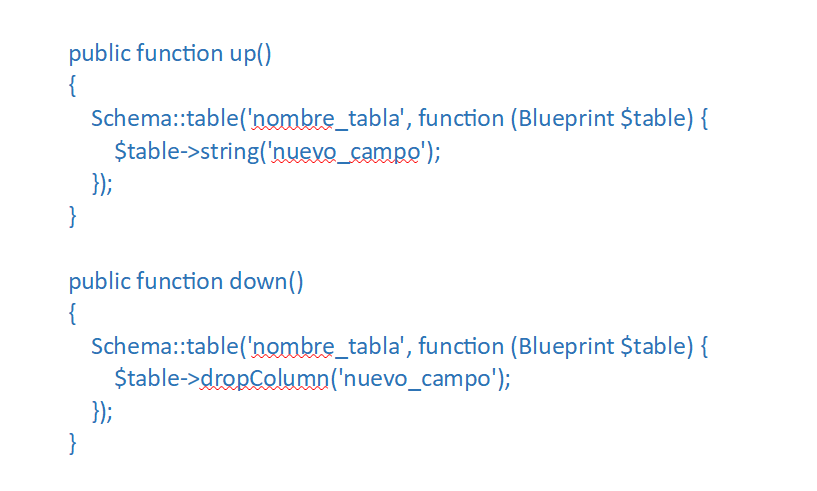
\includegraphics[width=12cm]{funcionesUpDown.png}
\caption{\label{fig:012} Funciones Up y Down}
\end{figure}

En el método \textbf{up()}, utilizamos el método \textbf{addColumn()} para agregar un nuevo campo a la tabla. En el método \textbf{down()}, utilizamos el método \textbf{dropColumn()} para revertir el cambio en caso de que sea necesario realizar una migración de rollback.
Ejecuta la migración: Una vez que hayas editado la migración, puedes ejecutar el comando \textbf{php artisan migrate} para aplicar los cambios en la tabla:\\

\textbf{bash}\\

\textbf{php artisan migrate}\\

Esto ejecutará todas las migraciones pendientes, incluyendo la nueva migración que hemos creado.
Laravel realizará los cambios en la tabla de acuerdo con la migración que hemos creado. Si necesitas realizar más modificaciones en la misma tabla, podemos crear migraciones adicionales y ejecutar el comando \textbf{php artisan migrate} para aplicar los cambios.
Las migraciones de Laravel permiten mantener un registro de los cambios realizados en la estructura de la base de datos y realizar actualizaciones de manera controlada. También puedes utilizar los comandos \textbf{php artisan migrate:rollback} y \textbf{php artisan migrate:refresh} para revertir o refrescar las migraciones, respectivamente.

\textbf{Deshacer migración:}
Una migración rollback (reversión de migración) en Laravel se refiere a deshacer los cambios realizados por una migración previamente ejecutada. Es una forma de revertir la última migración o un conjunto de migraciones a un estado anterior en la base de datos.
Cuando ejecutas una migración en Laravel, se realiza una modificación en la estructura de la base de datos, como crear una tabla, agregar un campo, modificar un índice, entre otros cambios. Si necesitas deshacer esos cambios, podemos utilizar el rollback.\\

\textbf{Creación de Controllers.}
Código ejemplo para crear un fichero controlador: 

\textbf{Php artisan make:controller Compras -resource}.

COOKIES:

Creamos un controller para nuestra página de Bienvenida

\textbf{php artisan make:controller WelcomeController - -resource}\\


\textbf{¿Cómo puedo ver qué paquetes están instalados?}
En el proyecto tenemos una carpeta llamada \textbf{vendor} que contiene todas las dependencias instaladas a través de \textbf{Composer}. Dentro de esta carpeta, se encuentra la carpeta correspondiente al paquete que deseamos verificar. Si encuentramos la carpeta del paquete, significa que está instalado.\\


\begin{figure}[!]
\centering
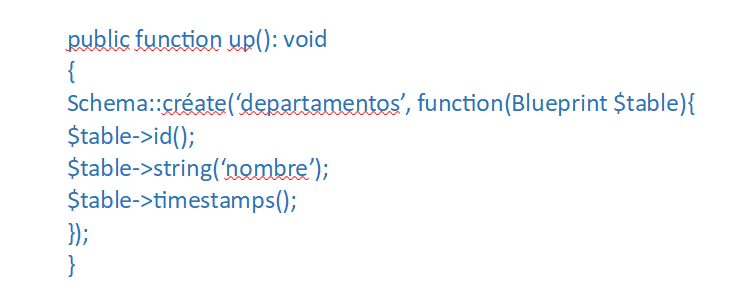
\includegraphics[width=12cm]{funciónCorrecciónError.png}
\caption{\label{fig:013} Funcion corregida que al principio daba error}
\end{figure}

\textbf{Session en Laravel.}
En Laravel, cuando se utiliza el sistema de autenticación `Auth` incorporado, se utiliza un mecanismo llamado ``tokens de autenticación'' para mantener la sesión del usuario. Estos tokens son almacenados en cookies o en el almacenamiento de sesión de Laravel.

Cuando un usuario inicia sesión en Laravel, se crea un token de autenticación único para ese usuario y se almacena en la sesión. Esta sesión se asocia con la cookie del navegador del usuario. Cuando el usuario realiza solicitudes posteriores al servidor, el token de autenticación se utiliza para verificar si el usuario está autenticado.

El comportamiento por defecto de Laravel es que un token de autenticación solo es válido para una única sesión o navegador. Esto significa que, si el usuario inicia sesión en un navegador y luego intenta abrir una sesión en otro navegador, el segundo inicio de sesión invalidará automáticamente el token de autenticación anterior, cerrando la sesión en el primer navegador.

\begin{figure}[!]
\centering
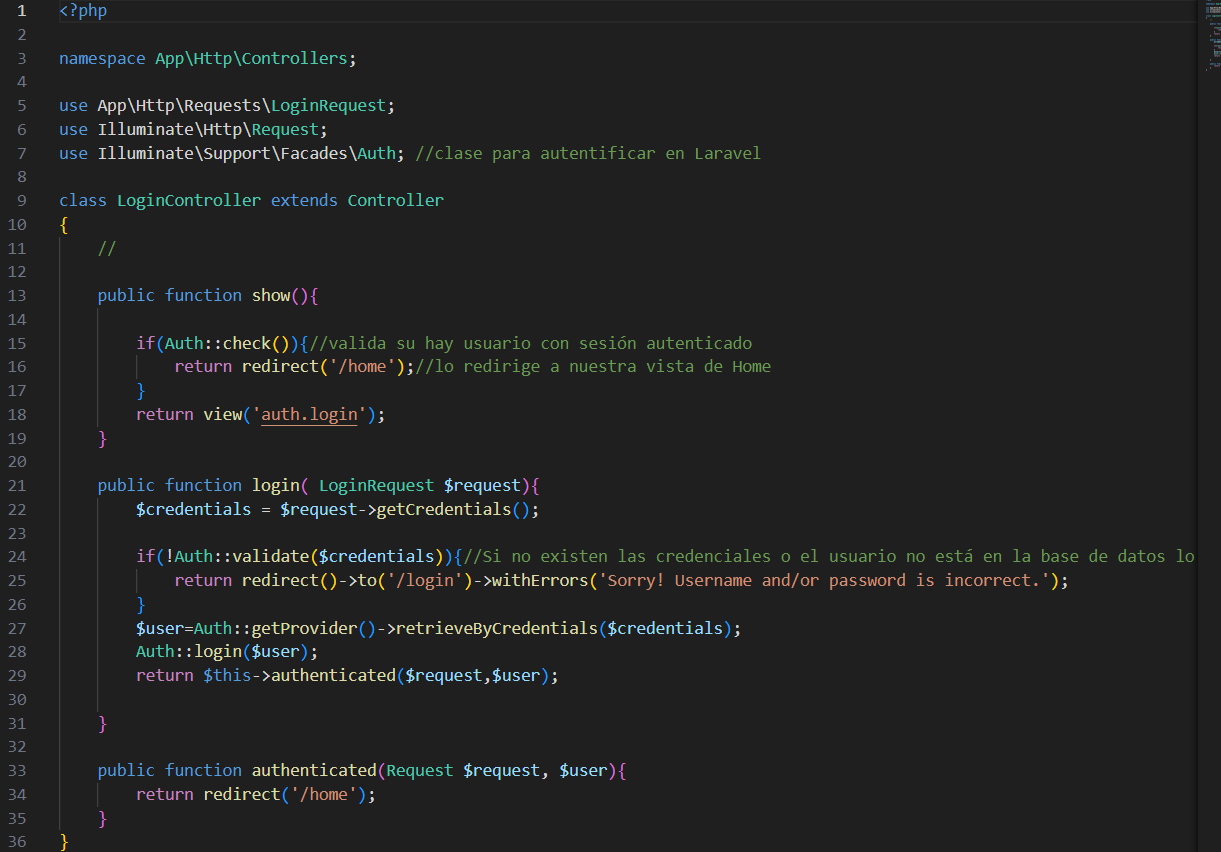
\includegraphics[width=12cm]{LoginController.png}
\caption{\label{fig:014} LoginController.php}
\end{figure}

Este comportamiento es controlado por Laravel a través del middleware ``StartSession'' y la configuración de sesión en ``config\/ session.php''.  La configuración ``driver'' en el archivo ``session.php'' determina dónde se almacenan las sesiones (por ejemplo, en archivos, en la base de datos, en Redis, etc.). Además, la opción ``same\_site'' puede configurarse para determinar si la cookie de sesión se puede compartir entre diferentes sitios o si se limita al mismo sitio. 

\begin{figure}[!]
\centering
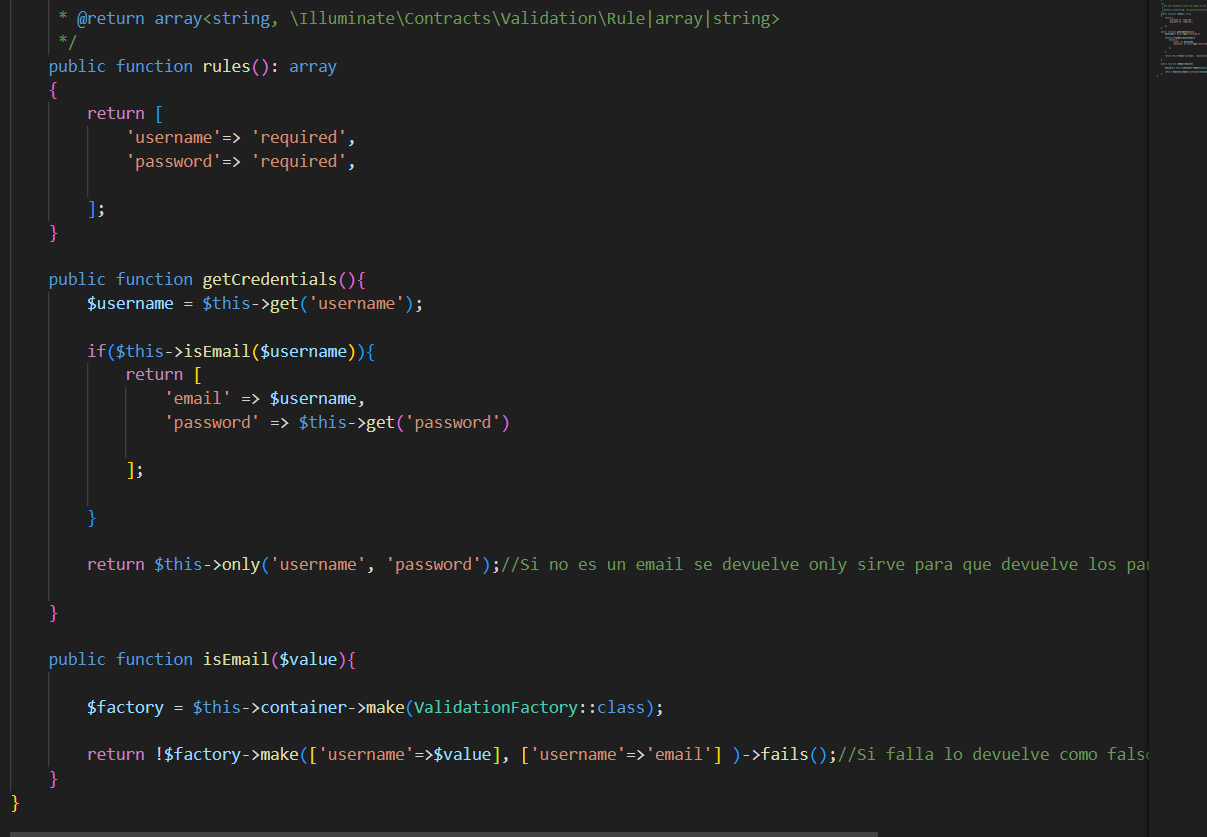
\includegraphics[width=12cm]{LoginRequest.png}
\caption{\label{fig:015} LoginRequest.php}
\end{figure}

Si queremos personalizar este comportamiento, podemos modificar el archivo ``session.php'' y ajustar la configuración según nuestras necesidades. Por ejemplo, podríamos permitir múltiples sesiones simultáneas configurando la opción ``expire\_on\_close'' a ``false'' y utilizando un driver de sesión compatible con múltiples sesiones, como la base de datos o Redis.

\begin{figure}[!]
\centering
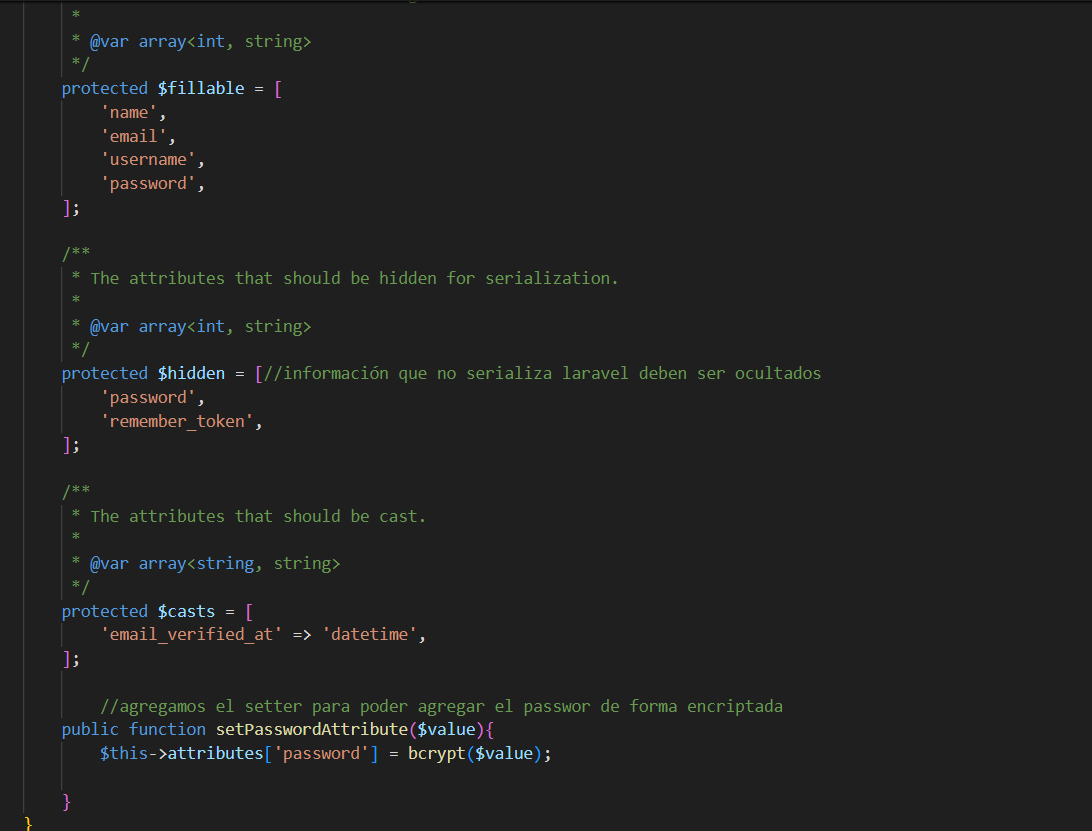
\includegraphics[width=12cm]{User.php(encriptado).png}
\caption{\label{fig:016} Configuración Encriptación}
\end{figure}

Es importante tener en cuenta que esta es la configuración predeterminada de Laravel, pero es posible modificarla o reemplazarla para adaptarse a tus requerimientos específicos de autenticación y sesiones.\\

\begin{figure}[!]
\centering
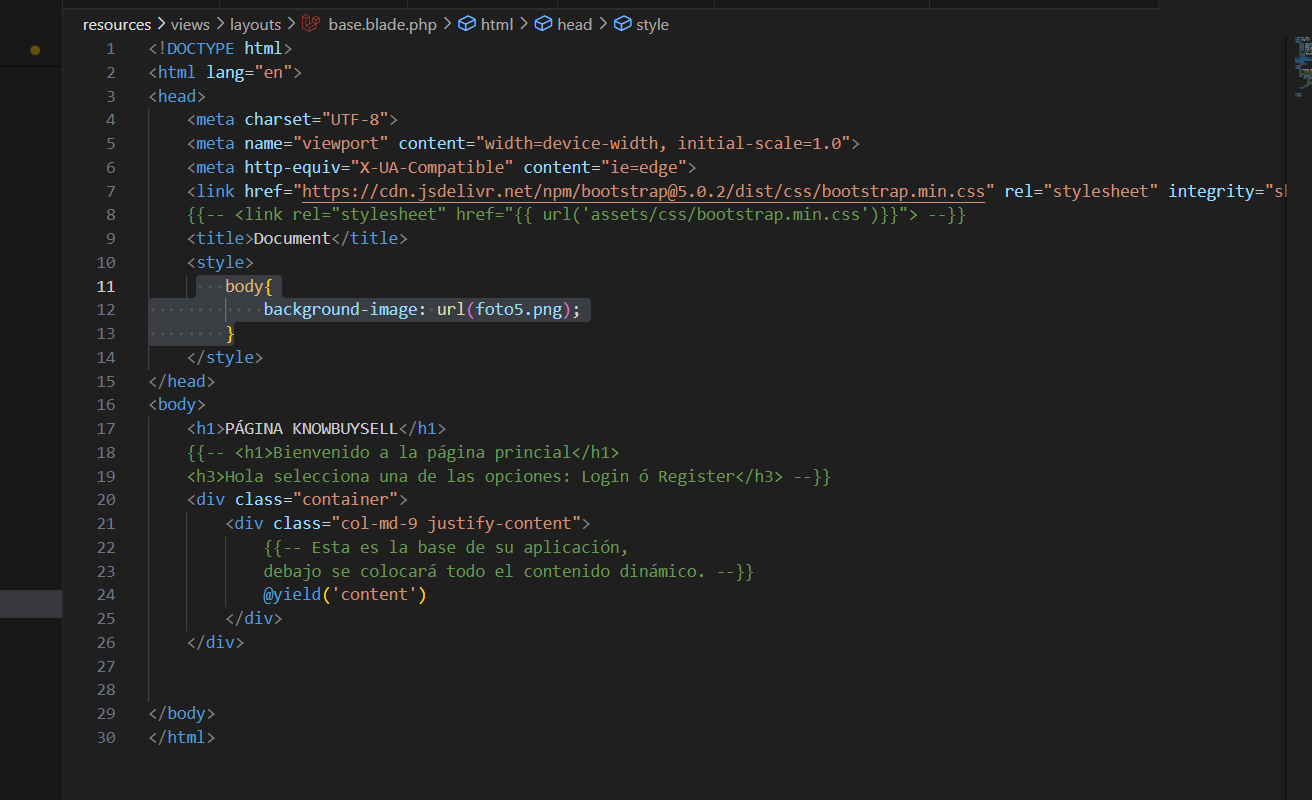
\includegraphics[width=12cm]{Base.blase(paginaPadre).png}
\caption{\label{fig:017} Página de la estructura básica, página padre de la que heredan el resto de páginas a través de @extends}
\end{figure}

\begin{figure}[!]
\centering
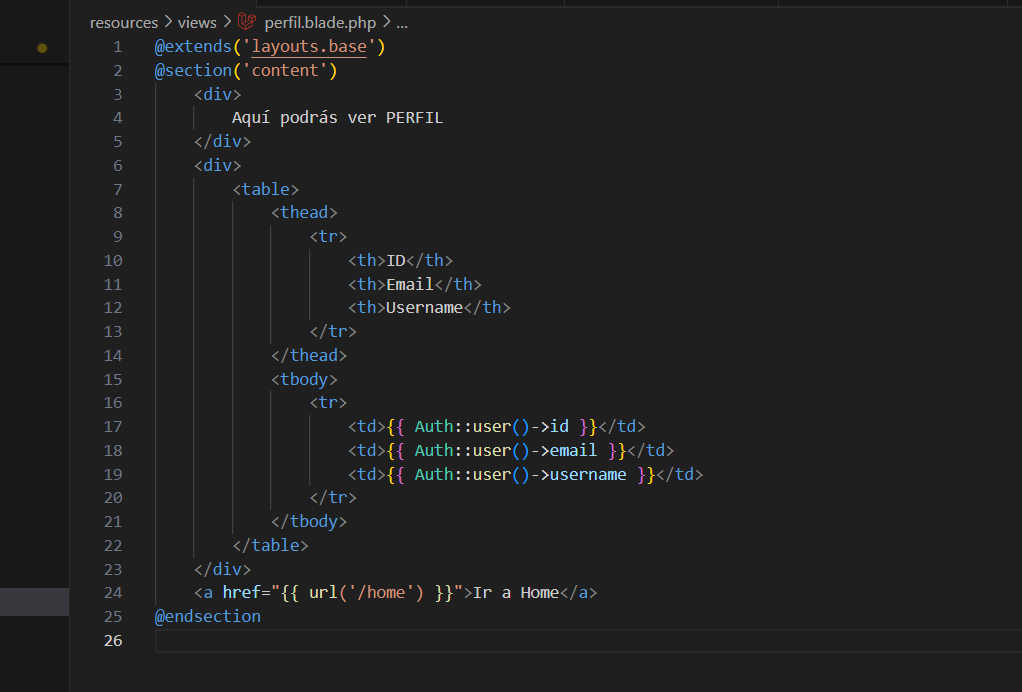
\includegraphics[width=12cm]{PerfilLogado(páginaHijo).png}
\caption{\label{fig:018} Página que hereda del padre su formato base}
\end{figure}

\textbf{Comprobar rutas activas.}
Podemos saber qué rutas tenemos activas a través del comando:\\

\textbf{Php artisan route:list}\\

Con este comando vemos los métodos y si se acede por POST etc… Para acción con la base de datos te indica qué método debemos usar.\\

\textbf{Reporte de errores solventados.}
\begin{enumerate}
    \item Importante: en las rutas tiene que estar bien identificado cada fichero de vistas.
    \item También es importante que se hagan las importaciones en el fichero de controlador de los paquetes o clases que tengamos que usar para que no nos dé fallo la aplicación.
    \item Instalé el paquete Breeze, pero lo tuve que desinstalar porque sospecho que no era compatible con otros paquetes que ya tenía instalados.
    \item Tuve que eliminar tablas a través de Laravel para poder corregir un error que me apareció.
    \item En el código de la Figura \ref{fig:013} también tuve error en la aplicación sólo porque se me había pasado incluir la palabra ‘nombre’ dentro de los paréntesis de string(), por lo que no me dejaba migrar la información. Ver Figura \ref{fig:013}

    \item Importante tener claro los campos de la base de datos para no tener que modificar tanto con las migraciones(descripcionproducto).
    \item Otros errores ya solventados.
\end{enumerate}


Las referencias \cite{DocumentaciónPHP} y \cite{DocumentaciónPHPManual} son útiles enlaces de Manuales consultados de PHP.
Libros consultados de PHP y MySQL: \cite{cursoPHP_2021} \cite{PHP_8} \cite{ProgAvanza}

\section{Algunos ejemplos de partes del código que considero más importantes o al menos curiosas porque las desconocía}

En la Figura \ref{fig:014} podemos ver cómo es la estructura de un controlador.\\

En la Figura \ref{fig:015} podemos comprobar la estructura del Login Request.\\

En la Figura \ref{fig:016} podemos comprobar cómo se ha configurado la encriptación del password.\\

En la Figura \ref{fig:017} podemos ver cómo hemos estructurado la base de la página padre, de esta heredarán el resto en el formato base.\\

En la Figura \ref{fig:018} en ella vemos cómo se realiza la herencia para el formato en este caso  a través de ``@extends(base)''.




\section{Conclusiones}
No ha sido fácil realizar la aplicación, ya que el concepto de mvc en un primer momento no me ha parecido demasiado fácil, ya que tienes que tener muy claro qué es y para qué es lo que estás haciendo en cada momento, pues finalmente es como si todo estuviera encadenado de una forma o de otra. Aunque el esquema para entender a priori el mvc parece fácil, una vez estás trabajando con Laravel, tienes que tener muy claro todo para que no empiecen a surgir errores. A pesar de ello he terminado satisfecha. Aunque reconozco que podría haber avazando más pero en cuanto a la parte de la gráfica he tenido más inconvenientes para poder finalizarla porque me ha costado más, aún no está correcta, pero seguiré trabajando en ello. 


Mi deseo es haber mejorado más la aplicación pero también es cierto, que compaginar trabajo con el desarrollo de la aplicación no es fácil, por eso estoy deseando poder trabajar como programadora y así poder rendir al máximo sin compaginar con otras obligaciones laborales.


Puedo estar satisfecha ya que al menos el programa funciona, de haber aprendido mucho, como es la configuración de cookies, login (el usuario mantienen la sesión abierta hasta que cierra el navegador), el usuario mete su clave y ésta queda encriptada en la base de datos, también hemos aprendido a configurar la creación de una cuenta, la sesión no se puede abrir en otro navegador pero si es el mismo se mantiene abierta, La conexión con la base de datos es correcta, hemos creado usuarios y se han almacenado en la base de datos de forma correcta, hemos realizado un CRUD en cuanto a las compras realizadas por los usuarios, cada usuario que entra puede crear una compra, modificar la compra y eliminar la compra, emos conseguido generar un documento pdf del listado de compras, hemos generado nuestros métodos que necesitábamos dentro del proyecto en PHP, he conseguido generar una gráfica según los datos, aunque hay que corregirla porque no está correcta, pero antes no salía y estuve mucho tiempo con el paquete en cuestión para crear la gráfica de los datos de la base de datos, y sobre todo por todo lo que he aprendido haciendo esta aplicación a pesar de que el lenguaje PHP con Laravel no es el que más me apasiona, volveré a intentar realizar mi proyecto en lenguaje JAVA o PYTHON, y terminaré de corregir algunas cosas.

También me gustaría poder incluir como \textbf{acciones de mejora} los productos con imágenes como cualquier página web, pero necesitaba hacerlo así para determinar bien el CRUD; y por falta de tiempo no lo pude complementar, otra mejora sería establecer las categorías como ENUM y que el sistema lo seleccione de forma automática cuando el usuario seleccione el producto a comprar, también tengo pendiente mejorar la gráfica para que puedan aparecer todas las categorías, todo ellos entre otras cosas a mejorar.

Finalmente quiero dar las gracias a todos los que me han apoyado y a todo aquel que haya invertido tiempo en leer esta documentación.¡Gracias!


\bibliographystyle{IEEEtran}
\bibliography{sample}
\end{document}